\chapter{Sample Production Details}

There's a lot of tuning which goes into sample production, involving things like trigger selections, MC validation checks, and of course writing code and creating bug fixes. There is a lot of work that goes into sample production (most of which is quite boring), but here I'm just going to talk about a few of the studies I did.

\section{Lepton Triggers}

One thing that goes into sample production is the selection of the trigger menu. We want to make sure that we choose triggers which capture most of the interesting objects, while not allowing an overwhelming amount of data to be present in our samples. Of course, we also select in such a way that the signal over background ratio for physics objects is maximized.

Here I show differences between four sets of trigger selections. First I describe the triggers that go into each menu, and then I compare trigger results in three different regions.

The trigger menus I will compare here are labelled 'trigMatch\_1L2LTrig', 'trigMatch\_1L2LTrigOR', 'trigMatch\_2LTrig', and 'trigMatch\_2LTrigOR'. The difference between 1L2LTrig and 2LTrig menus is that 1L2LTrig menus contain both single-lepton triggers like HLT\_e60\_medium and two-lepton triggers like HLT\_2mu10 while the 2LTrig menus only contain the two-lepton triggers. The difference between OR and non-OR menus is that the non-OR menus use the lowest unprescaled triggers in each run, while the OR menus use all triggers over all runs. The OR triggers are easier to implement and debug. Low-\pt\ isolated single-lepton triggers are not included, since they would bias the estimation of fake leptons using the matrix method (as will be described in the next chapter). High-\pt\ non-isolated single-lepton triggers are also not included, since they make scale factor calculation more complicated, and were found not to increase signal acceptance by very much.

Using data and a selection of signal samples (taken from an electroweak model sample grid), we look at trigger efficiencies in several regions. In Tables~\ref{tab:trigger_first} to~\ref{tab:trigger_last} we quote the percentage of events which pass each trigger in each region, using all events in that region (with no trigger requirement) as a baseline. We found that 2LTrigOR was a good menu to use, as it maintained a good signal over background ratio, while being the simplest to implement. Values in these tables are labelled `nan` when there are no passing events.

\begin{table}
\begin{center}
\caption{trigMatch\_1L2LTrig Efficiency in SR Low Region (\%)}
\begin{tabular}{l|l|l}
& ee & mm \\
\hline
data15-16 & 100 & 93.9655 \\
data17 & 82.6087 & 84.507 \\
data18 & 91.3044 & 79.375 \\
(600, 0) MC16a & 100 & 100 \\
(600, 0) MC16cd & 100 & 100 \\
(600, 0) MC16e & 100 & 83.3333 \\
(200, 100) MC16a & -nan & -nan \\
(200, 100) MC16cd & -nan & -nan \\
(200, 100) MC16e & -nan & -nan
\label{tab:trigger_first}
\end{tabular}
\end{center}
\end{table}

\begin{table}
\begin{center}
\caption{trigMatch\_1L2LTrigOR Efficiency in SR Low Region (\%)}
\begin{tabular}{l|l|l}
& ee & mm \\
\hline
data15-16 & 100 & 95.6897 \\
data17 & 82.6087 & 97.1831 \\
data18 & 91.3044 & 96.25 \\
(600, 0) MC16a & 100 & 100 \\
(600, 0) MC16cd & 100 & 100 \\
(600, 0) MC16e & 100 & 100 \\
(200, 100) MC16a & -nan & -nan \\
(200, 100) MC16cd & -nan & -nan \\
(200, 100) MC16e & -nan & -nan \\
\end{tabular}
\end{center}
\end{table}

\begin{table}
\begin{center}
\caption{trigMatch\_2LTrig Efficiency in SR Low Region (\%)}
\begin{tabular}{l|l|l}
& ee & mm \\
\hline
data15-16 & 84.6154 & 90.5172 \\
data17 & 78.2609 & 92.9577 \\
data18 & 65.2174 & 93.125 \\
(600, 0) MC16a & 100 & 100 \\
(600, 0) MC16cd & 66.6667 & 88.8889 \\
(600, 0) MC16e & 100 & 100 \\
(200, 100) MC16a & -nan & -nan \\
(200, 100) MC16cd & -nan & -nan \\
(200, 100) MC16e & -nan & -nan \\
\end{tabular}
\end{center}
\end{table}

\begin{table}
\begin{center}
\caption{trigMatch\_2LTrigOR Efficiency in SR Low Region (\%)}
\begin{tabular}{l|l|l}
& ee & mm \\
\hline
data15-16 & 84.6154 & 90.5172 \\
data17 & 78.2609 & 92.9577 \\
data18 & 65.2174 & 93.125 \\
(600, 0) MC16a & 100 & 100 \\
(600, 0) MC16cd & 66.6667 & 88.8889 \\
(600, 0) MC16e & 100 & 100 \\
(200, 100) MC16a & -nan & -nan \\
(200, 100) MC16cd & -nan & -nan \\
(200, 100) MC16e & -nan & -nan \\
\end{tabular}
\end{center}
\end{table}

\begin{table}
\begin{center}
\caption{trigMatch\_1L2LTrig Efficiency in SR Medium Region (\%)}
\begin{tabular}{l|l|l}
& ee & mm \\
\hline
data15-16 & 100 & 92.4242 \\
data17 & 86.2069 & 88 \\
data18 & 97.7273 & 83.0769 \\
(600, 0) MC16a & 99.6942 & 98.5795 \\
(600, 0) MC16cd & 99.6528 & 97.2973 \\
(600, 0) MC16e & 99.6169 & 96.3636 \\
(200, 100) MC16a & -nan & 100 \\
(200, 100) MC16cd & 100 & 100 \\
(200, 100) MC16e & 100 & -nan \\
\end{tabular}
\end{center}
\end{table}

\begin{table}
\begin{center}
\caption{trigMatch\_1L2LTrigOR Efficiency in SR Medium Region (\%)}
\begin{tabular}{l|l|l}
& ee & mm \\
\hline
data15-16 & 100 & 93.9394 \\
data17 & 86.2069 & 96 \\
data18 & 97.7273 & 91.5385 \\
(600, 0) MC16a & 100 & 98.8636 \\
(600, 0) MC16cd & 99.6528 & 99.6997 \\
(600, 0) MC16e & 99.6169 & 99.0909 \\
(200, 100) MC16a & -nan & 100 \\
(200, 100) MC16cd & 100 & 100 \\
(200, 100) MC16e & 100 & -nan \\
\end{tabular}
\end{center}
\end{table}

\begin{table}
\begin{center}
\caption{trigMatch\_2LTrig Efficiency in SR Medium Region (\%)}
\begin{tabular}{l|l|l}
& ee & mm \\
\hline
data15-16 & 91.6667 & 90.9091 \\
data17 & 79.3103 & 92 \\
data18 & 84.0909 & 86.1538 \\
(600, 0) MC16a & 97.5535 & 97.1591 \\
(600, 0) MC16cd & 94.4444 & 96.6967 \\
(600, 0) MC16e & 94.636 & 97.5758 \\
(200, 100) MC16a & -nan & 100 \\
(200, 100) MC16cd & 100 & 100 \\
(200, 100) MC16e & 100 & -nan \\
\end{tabular}
\end{center}
\end{table}

\begin{table}
\begin{center}
\caption{trigMatch\_2LTrigOR Efficiency in SR Medium Region (\%)}
\begin{tabular}{l|l|l}
& ee & mm \\
\hline
data15-16 & 95.8333 & 90.9091 \\
data17 & 79.3103 & 92 \\
data18 & 84.0909 & 86.1538 \\
(600, 0) MC16a & 97.5535 & 97.1591 \\
(600, 0) MC16cd & 94.4444 & 96.6967 \\
(600, 0) MC16e & 94.636 & 97.5758 \\
(200, 100) MC16a & -nan & 100 \\
(200, 100) MC16cd & 100 & 100 \\
(200, 100) MC16e & 100 & -nan \\
\end{tabular}
\end{center}
\end{table}

\begin{table}
\begin{center}
\caption{trigMatch\_1L2LTrig Efficiency in SR High Region (\%)}
\begin{tabular}{l|l|l}
& ee & mm \\
\hline
data15-16 & 100 & 92.3077 \\
data17 & 100 & 72.7273 \\
data18 & 50 & 57.1429 \\
(600, 0) MC16a & 100 & 94.1176 \\
(600, 0) MC16cd & 100 & 90.9091 \\
(600, 0) MC16e & 90 & 100 \\
(200, 100) MC16a & -nan & -nan \\
(200, 100) MC16cd & -nan & -nan \\
(200, 100) MC16e & 100 & -nan \\
\end{tabular}
\end{center}
\end{table}

\begin{table}
\begin{center}
\caption{trigMatch\_1L2LTrigOR Efficiency in SR High Region (\%)}
\begin{tabular}{l|l|l}
& ee & mm \\
\hline
data15-16 & 100 & 92.3077 \\
data17 & 100 & 81.8182 \\
data18 & 50 & 66.6667 \\
(600, 0) MC16a & 100 & 94.1176 \\
(600, 0) MC16cd & 100 & 90.9091 \\
(600, 0) MC16e & 90 & 100 \\
(200, 100) MC16a & -nan & -nan \\
(200, 100) MC16cd & -nan & -nan \\
(200, 100) MC16e & 100 & -nan \\
\end{tabular}
\end{center}
\end{table}

\begin{table}
\begin{center}
\caption{trigMatch\_2LTrig Efficiency in SR High Region (\%)}
\begin{tabular}{l|l|l}
& ee & mm \\
\hline
data15-16 & 100 & 92.3077 \\
data17 & 100 & 81.8182 \\
data18 & 50 & 66.6667 \\
(600, 0) MC16a & 100 & 94.1176 \\
(600, 0) MC16cd & 85.7143 & 90.9091 \\
(600, 0) MC16e & 90 & 100 \\
(200, 100) MC16a & -nan & -nan \\
(200, 100) MC16cd & -nan & -nan \\
(200, 100) MC16e & 100 & -nan \\
\end{tabular}
\end{center}
\end{table}

\begin{table}
\begin{center}
\caption{trigMatch\_2LTrigOR Efficiency in SR High Region (\%)}
\begin{tabular}{l|l|l}
& ee & mm \\
\hline
data15-16 & 100 & 92.3077 \\
data17 & 100 & 81.8182 \\
data18 & 50 & 66.6667 \\
(600, 0) MC16a & 100 & 94.1176 \\
(600, 0) MC16cd & 85.7143 & 90.9091 \\
(600, 0) MC16e & 90 & 100 \\
(200, 100) MC16a & -nan & -nan \\
(200, 100) MC16cd & -nan & -nan \\
(200, 100) MC16e & 100 & -nan
\label{tab:trigger_last}
\end{tabular}
\end{center}
\end{table}

\section{MC Angle Validation Plots}

Part of MC validation involves checking for any deadspots or hotspots in the 2D eta-phi angle space~\cite{twiki_checks} for leading jets and leptons. Any large peaks or dips would demonstrate an issue in the sample production process. To do these checks, I created plots for our various sample processes in each of our strong and electroweak regions.

A random selection of these plots are shown in Figures~\ref{fig:MC_angle_validation_first} to~\ref{fig:MC_angle_validation_last}. Examining these plots demonstrated that there were no issues in this particular case.

\begin{figure}[htbp]
\centering
\begin{minipage}{0.45\textwidth}
    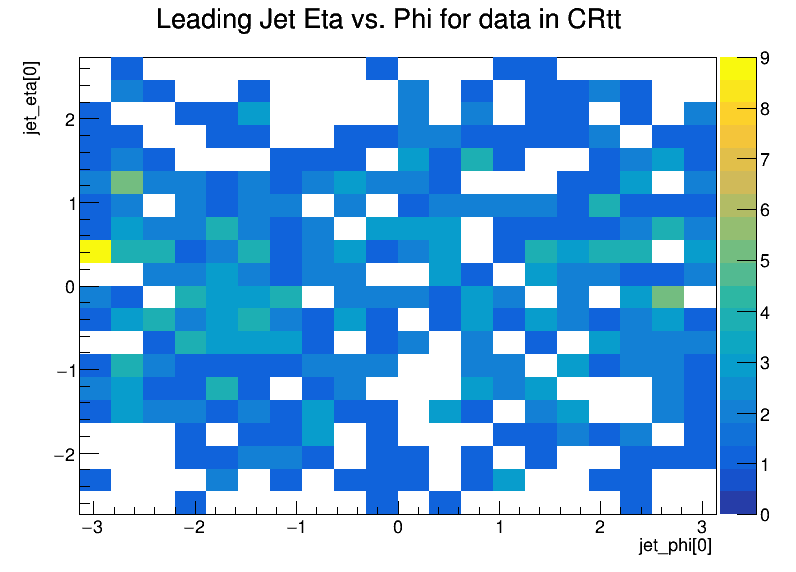
\includegraphics[width=\textwidth]{Images/SUSY/jet_eta_phi_data_CRtt.png}
    \caption{$\eta$ vs $\phi$ plot for leading jets for data in CRtt.}
    \label{fig:MC_angle_validation_first}
\end{minipage}
\hfill
\begin{minipage}{0.45\textwidth}
    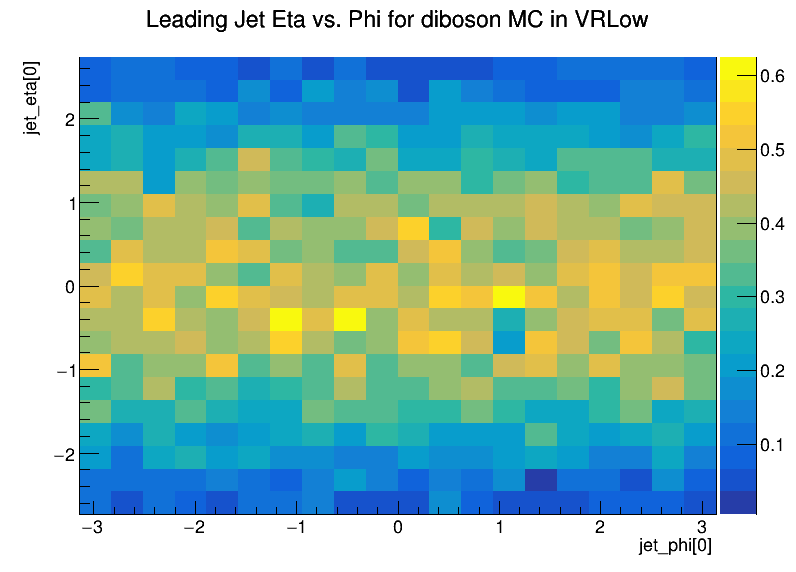
\includegraphics[width=\textwidth]{Images/SUSY/jet_eta_phi_diboson_VRLow.png}
    \caption{$\eta$ vs $\phi$ plot for leading jets for diboson in VRLow.}
\end{minipage}
\end{figure}

\begin{figure}[htbp]
\centering
\begin{minipage}{0.45\textwidth}
    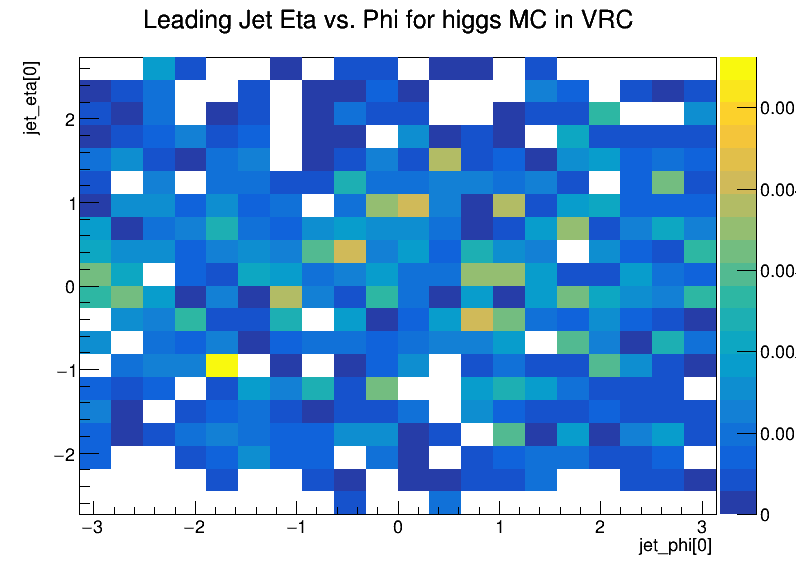
\includegraphics[width=\textwidth]{Images/SUSY/jet_eta_phi_higgs_VRC.png}
    \caption{$\eta$ vs $\phi$ plot for leading jets for higgs in VRC.}
\end{minipage}
\hfill
\begin{minipage}{0.45\textwidth}
    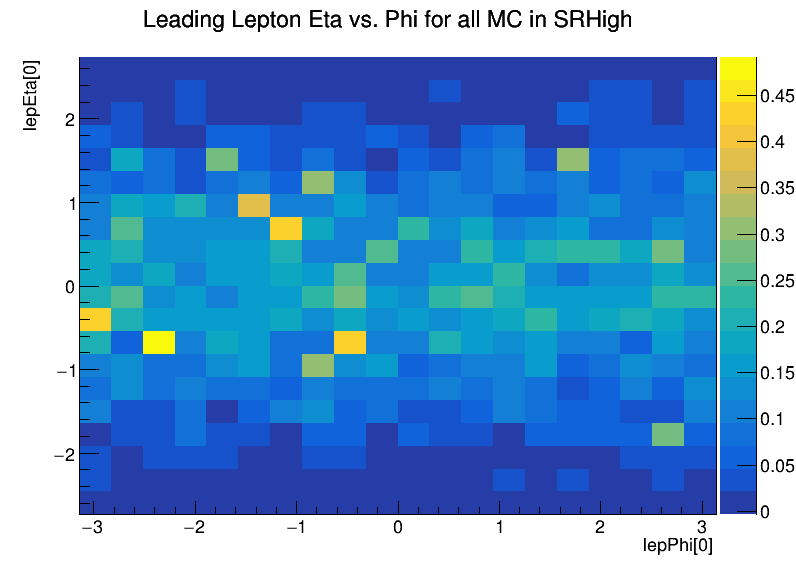
\includegraphics[width=\textwidth]{Images/SUSY/lep_eta_phi_all_MC_SRHigh.png}
    \caption{$\eta$ vs $\phi$ plot for leading leptons for all MC in SRHigh.}
\end{minipage}
\end{figure}

\begin{figure}[htbp]
\centering
\begin{minipage}{0.45\textwidth}
    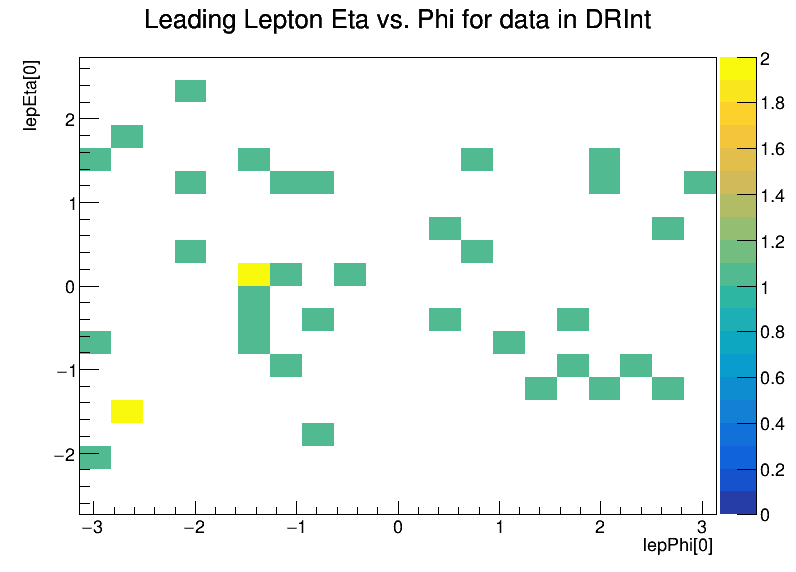
\includegraphics[width=\textwidth]{Images/SUSY/lep_eta_phi_data_DRInt.png}
    \caption{$\eta$ vs $\phi$ plot for leading leptons for data in DRInt.}
\end{minipage}
\hfill
\begin{minipage}{0.45\textwidth}
    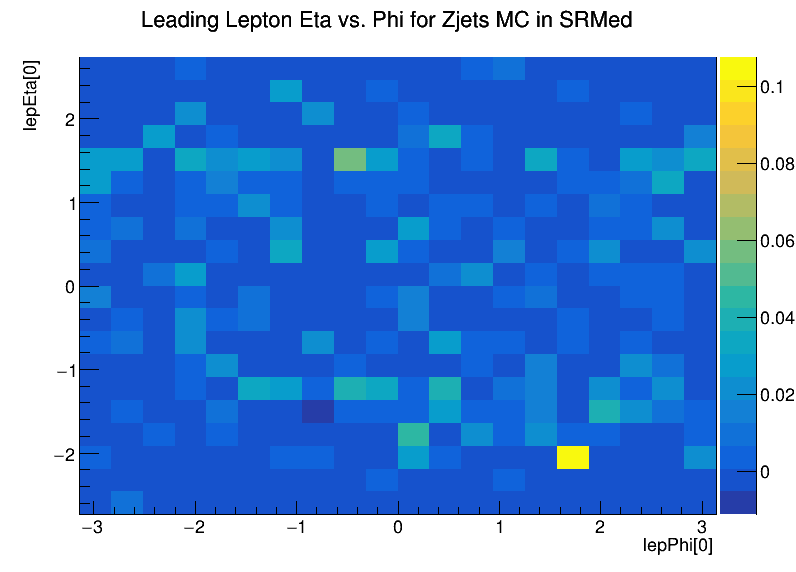
\includegraphics[width=\textwidth]{Images/SUSY/lep_eta_phi_Zjets_SRMed.png}
    \caption{$\eta$ vs $\phi$ plot for leading lepton for Zjets in SRMed.}
    \label{fig:MC_angle_validation_last}
\end{minipage}
\end{figure}

\section{\ptll\ Cut}

Here we look at the effect of a \ptll\ cut on signal and data. Specifically, we see what happens if we take a baseline selection of at least two jets (with \pt\ above 30 GeV), at least two leptons (with \pt\ above 25 GeV), and \MET\ above 200 GeV, and add a \ptll$>40$ GeV cut.

In Figure~\ref{fig:ptll_cut}, we look at an MC16e SLN1 sample grid. These are electroweak samples, but they behave similarly to the strong model samples. Here we look at events which have already passed the baseline selection, and see how many of them would pass an additional \ptll\ cut. Furthermore, we compare them with the passing efficiency numbers for all background processes (as simulated by MC), and for the largest background, ttbar, in Table~\ref{tab:ptll_cut}. We see that the \ptll\ cut removes more background than signal over most of the grid. For this reason we added the \ptll$>40$ cut to our baseline selection.

\begin{figure}[htbp]
    \centering
    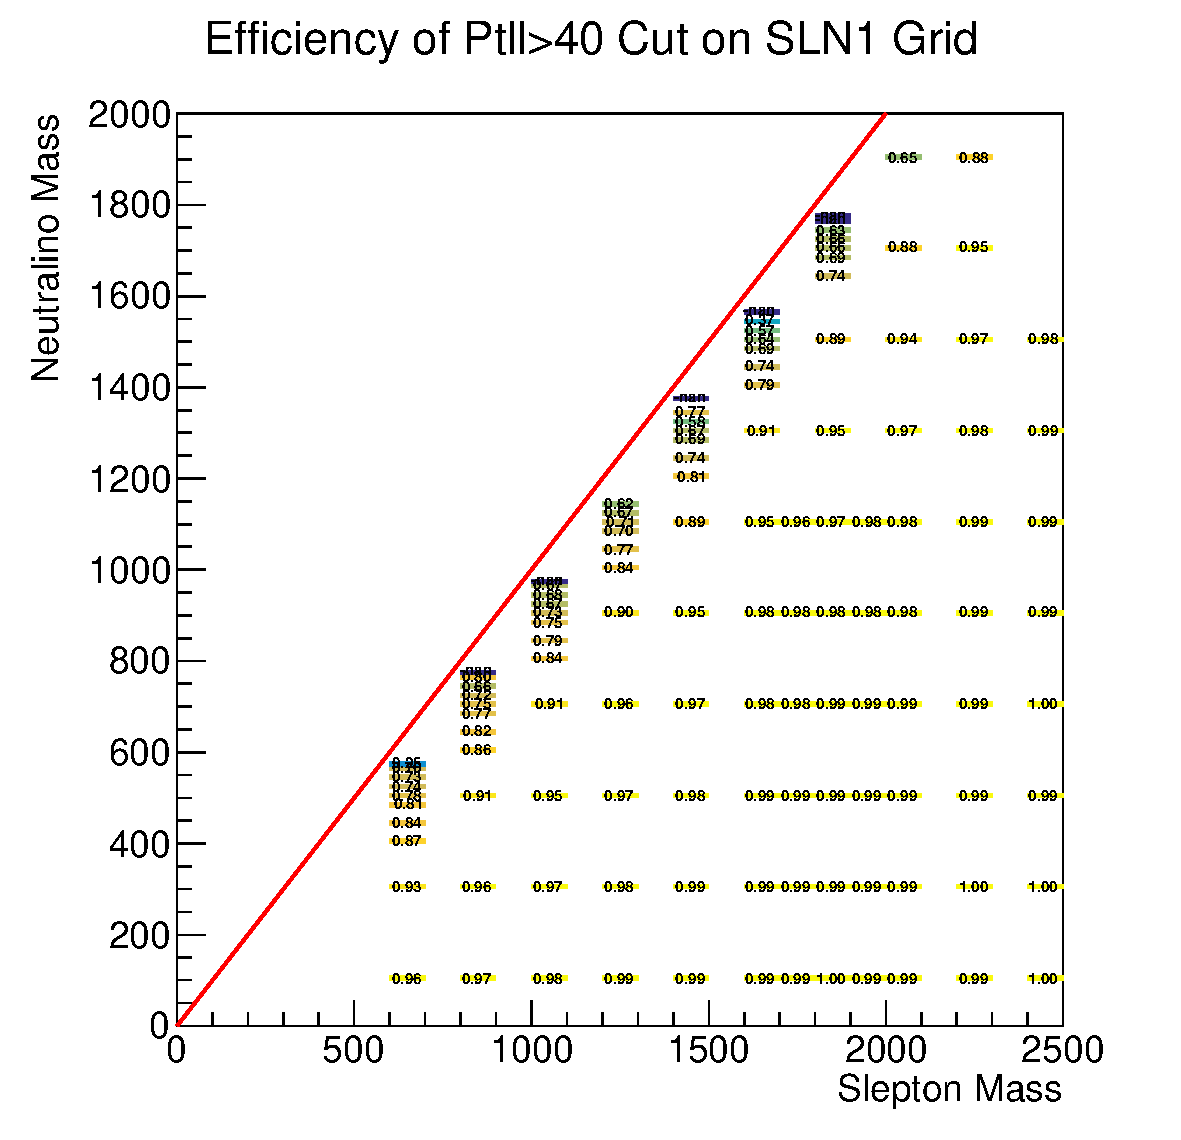
\includegraphics[width=0.85\textwidth]{Images/SUSY/ptll_cut_efficiency.pdf}
    \caption{Efficiency of a \ptll\ cut on the SLN1 signal grid.}
    \label{fig:ptll_cut}
\end{figure}

\begin{table}[htbp]
\caption{\ptll\ Cut Efficiency}
\begin{center}
\begin{tabular}{c|c|c|c}
& mc16a & mc16cd & mc16e \\
\hline
ttbar & 0.866 & 0.883 & 0.881 \\
all MC & 0.881 & 0.904 & 0.896 \\
\end{tabular}
\end{center}
\label{tab:ptll_cut} 
\end{table}

\section{Photon Overlap Removal}

Another issue we had to check was the use of overlap removal in sample production. After the photon method (to be described later) was shown to be problematic, we turned off photon-based overlap removal for the next set of samples. Here I show that this choice did not have a significant impact on relevant Z and data samples.

To do this, I checked a subset of samples for Z MC and data. I produced these samples with and without the OR.DoPhoton flag, and plotted the \MET\ distributions against each other. These plots, shown in Figures~\ref{fig:ORPhoton_first} to~\ref{fig:ORPhoton_last}, demonstrates that turning off photon overlap removal does not have much impact.

The samples used are the following:

\begin{itemize}
    \item \seqsplit{mc16\_13TeV.364121.Sherpa\_221\_NNPDF30NNLO\_Zee\_MAXHTPTV140\_280\_CFilterBVeto.deriv.DAOD\_SUSY2.e5299\_s3126\_r10724\_p4189}
    \item \seqsplit{mc16\_13TeV.364102.Sherpa\_221\_NNPDF30NNLO\_Zmumu\_MAXHTPTV0\_70\_BFilter.deriv.DAOD\_SUSY2.e5271\_s3126\_r10201\_p4189}
    \item \seqsplit{data18\_13TeV.periodB.physics\_Main.PhysCont.DAOD\_SUSY2.grp18\_v01\_p3991}.
\end{itemize}

\begin{figure}[htbp]
\centering
\begin{minipage}{0.45\textwidth}
    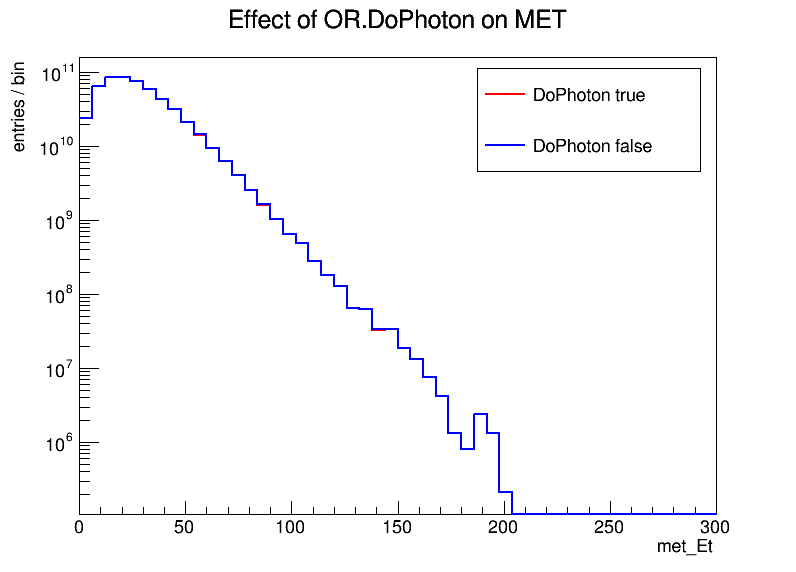
\includegraphics[width=\textwidth]{Images/SUSY/ORDoPhoton_Zee.png}
    \caption{\MET\ with and without photon overlap removal for Zee.}
    \label{fig:ORPhoton_first}
\end{minipage}
\hfill
\begin{minipage}{0.45\textwidth}
    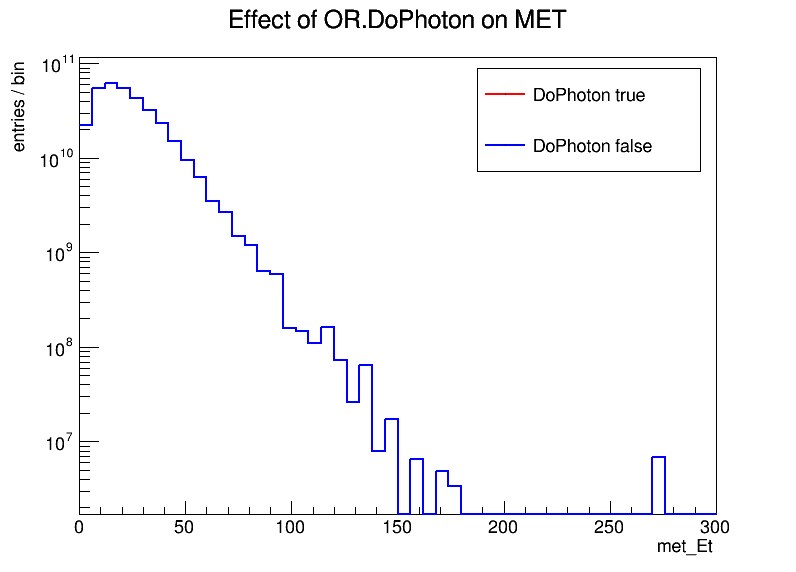
\includegraphics[width=\textwidth]{Images/SUSY/ORDoPhoton_Zmm.png}
    \caption{\MET\ with and without photon overlap removal for Zmm.}
\end{minipage}
\end{figure}

\begin{figure}[htbp]
    \centering
    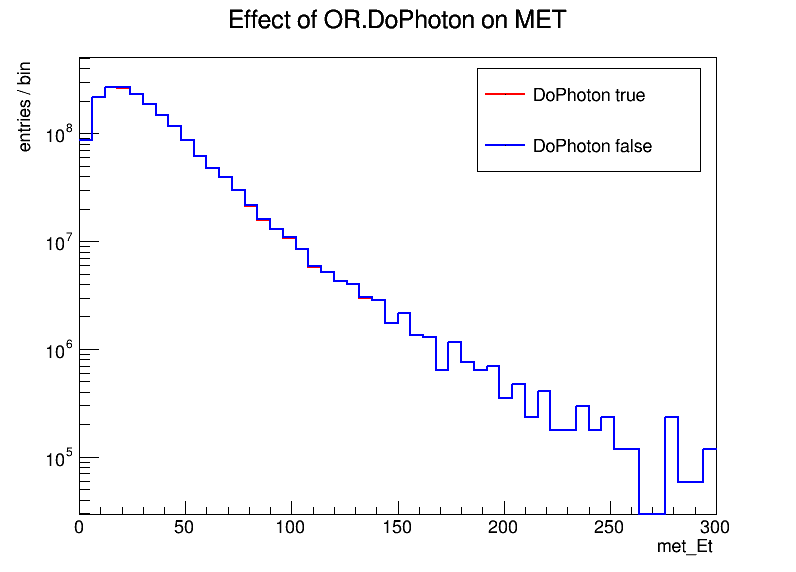
\includegraphics[width=0.45\textwidth]{Images/SUSY/ORDoPhoton_data.png}
    \caption{\MET\ with and without photon overlap removal for data.}
    \label{fig:ORPhoton_last}
\end{figure}